\chapter{熵表象下的统计力学:微正则系综}
\label{chap15}
{\it (译者注:原文所有的`formalism'翻译为“系综”。如`microcanonical formalism'译作“微正则系综”。)}

\section{封闭系统的熵的物理意义}
热力学是普适而有力的理论体系,并且只以几个简单假设为基础。熵在热力学假设中处于核心地位,它是作为极值原理决定平衡态的抽象数学函数引入的,然而在之后的理论中,熵与能量、体积、摩尔数、磁矩等物理量一样,是系统的广延量。后面几个量都有清晰而基础的物理意义,而熵在其中显得格格不入。

统计力学诠释了熵的物理意义,从而为极值原理提供了启发性的论证。对于一些有解析解的简单系统,这种诠释能够直接计算熵,于是也得出了基本方程。

首先考虑一个体积、粒子数固定的封闭系统,为了明确起见不妨认为其中是液体(别的也可以)。系统的限制条件是参量$U, V, N$的值不变,量子力学表明,微观系统\mpar{原文为“macroscopic”(宏观系统),显然与下文不符(能级量子化是微观系统的特性),怀疑此处为笔误,译文进行了修改。}给定的$U, V, N$可以对应多个分立的量子态,系统可能处于这些状态中的任何一个。

人们也许天真地以为,初始位于某个定态\mpar{即Schrodinger方程的能量本征解。}的系统将永远保持那个状态,实际上这就是量子力学入门课告诉我们的;表面上看,指定了特定状态的“量子数”是“运动常数”。这一简单的“虚构”看法在研究微观原子系统(这也是量子力学应用最广的领域)尚可接受,而在研究宏观系统时则大错特错。

这一显然的悖论源自物理系统的{\it 孤立性}假设。{\it 没有任何物理系统是真正孤立的。} 微弱而长程的引力、电磁力等等充满了整个空间,不仅空间上分离的两个系统有力的作用,而且力场{\it 自身}是一种物理系统、参加与“孤立系统”的相互作用。真空现在被认为是具有复杂涨落实体——在其中不断发生着电子、正电子、中微子以及其他无数神秘的亚原子实体产生、再吸收的过程。所有这些事件都可以与“孤立系统”发生耦合。

对于简单系统(例如氢原子),上面提及的微弱相互作用几乎不会引起量子态的跃迁。因为氢原子等等系统量子态的能量范围较大,空间中微弱的随机相互作用提供不了这么大的能量使能级改变。即便如此,这种“几乎不会”的过程还是可以发生的,一个处于激发态的原子会“自发”发射一个光子,然后衰变到低能态。量子场论揭示了这种表面上“自发”的跃迁实际上是激发态原子与真空模式相互作用而{\it 诱发}的结果。这种原子{\it 不会}无限长的处于一个态,因为它会与真空模式进行相互作用。

宏观系统的量子态是连续的,各能级之差是微小的。对于大量原子组成的宏观系统,单个原子的能量本征态“分裂”成系统的$10^{23}$个本征态,因此平均的能级差减小了$\sim 10^{23}$倍。这样,即使最微弱的随机相互作用场或者真空涨落的微弱耦合也能够让系统在不同状态之间演化。

{\it 
更加真实的看法是,宏观系统在它可能的各量子态之间不断进行随机、迅速的跃迁。宏观测量只能测到无数量子态的平均性质。

{\bf 原文:} A realistic view of a macroscopic system is one in which the system makes enormously rapid random transitions among its quantum states. A macroscopic measurement senses only an average of the properties of myriads of quantum states.
}

所有“统计力学学家”都同意上一段的结论,然而在诱发跃迁的{\it 主要的}物理机制上有分歧。不同的物理机制相互竞争,有的机制也许在某些甚至所有系统中都居主导地位。这些都无所谓——任何机制都行,只要保证系统在量子态之间的跃迁是随机、迅速的就好了,统计力学理论只要求这一点。

既然这种跃迁是随机发生的,那么很可以假设{\it 宏观系统处于任意可能的状态的概率相等}——“可能的状态”是指系统在外部约束下可以处于的状态。

系统处于所有可能微观态的等概率假设是统计力学的基本假设。第III部分将进一步探究它的可靠性,现在只要接受就可以了,它具有先验的合理性,从它导出的结论大获成功。

假设系统的某些限制被移除,例如打开阀门让系统膨胀至更大体积。从微观层面看,移除限制的过程使得原来某些不可达到的微观态变得可以达到,系统可以在这些新的可能状态之间跃迁。一段时间后,新旧状态的差别就消失了,系统在{\it 增广了的}状态集合里等概率随机跃迁。{\it 微观态数目增长到相应限制之下的最大值。}\mpar{原文:The number of microstates among which the system undergoes transitions, and which thereby share uniform probability of occupation, increases to the maximum permitted by the imposed constraints. 原文意思有所重复,译文进行删减。}

这与热力学里面熵的假设太像了!热力学假设熵在给定约束下取最大值。这暗示着熵与宏观约束相应的微观态数目是一回事。

但是有个问题:熵是广延量,具有可加性,而微观态数目是相乘的。即复合系统的微观态数为子系统状态数的乘积(例如两个骰子的“微观态”数为$6 \times 6 = 36$)。为了用微观态数目解释熵,我们得定义一个与状态数有关的、可加性的量。(唯一的!)答案是微观态数目的对数(乘积的对数等于各因子对数之和),即
\begin{equation}
	S = k_B \ln \Omega.
\label{equ15.1}
\end{equation}
其中$\Omega$表示宏观约束相应的微观态数目。常数因子$k_B$(称为Boltzmann常数)仅仅用来决定$S$的取值,通常定义与温度的Kelvin温标一致,即$T^{-1} = \partial S / \partial U$. 后面会看到这要求$k_B = R/N_A = 1.3807 \times 10^{-23} \, \mathrm{J/K}$.

{\it 熵的定义式\eqref{equ15.1}是统计力学的基础。}

就像热力学在Legendre变换的处理下更加便利那样,上面的这个额外假设用类似的数学理论加以处理会更有效,当然即使不这样处理,这个简洁的新假设也是完备的,足以发展出统计力学理论。直接应用该假设,也就是直接计算系统可能的状态数目的对数,原则上能算出$S$关于宏观限制$U, V, N$的函数,这就是熵表象下的统计力学,或者用场论的说法,是{\it 微正则系综 (microcanonical formalism)}\mpar{“系综”的英文为“ensemble”,为了与其他教材说法一致我们将“xx formalism”都译成了“xx系综”。}之中的统计力学。 

本章其余几节要处理一系列微正则系综的例子,从而说明新假设的完备性。

就像热力学当中熵表象并不总是最方便的表象那样,统计力学的微正则系综经常是没有解析解的。通常要用到Legendre表象变换,这在下一章讲述。即使如此,微正则系综仍然建立起统计力学清晰、基本的逻辑基础。

\subsection*{习题}
\begin{itemize}
\item[15.1-1.] A system is composed of two harmonic oscillators each of natural frequency $\omega_0$ and each having permissible energies $(n + \dfrac{1}{2}) \hbar \omega$, where $n$ is any non-negative integer. The total energy of the system is $E' = n' \hbar \omega$, where $n'$ is a
positive integer. How many microstates are available to the system? What is the entropy of the system?

A second system is also composed of two harmonic oscillators, each of natural frequency $2\omega_0$. The total energy of this system is $E'' = n'' \hbar \omega_0$, where $n''$ is an even integer. How many microstates are available to this system? What is the entropy of this system? 

What is the entropy of the system composed of the two preceding subsystems (separated and enclosed by a totally restrictive wall)? Express the entropy as a function of $E'$ and $E''$.

\begin{flushright}
{\it Answer:}

${\displaystyle S_{\text{tot}} = k_B \ln \left( \frac{E' E''}{2\hbar^2 \omega_0^2} \right) }$
\end{flushright}

\item[15.1-2.] A system is composed of two harmonic oscillators of natural frequencies $\omega_0$ and 2$\omega_0$, respectively. If the system has total energy $E = (n + \dfrac{1}{2}) \hbar \omega_0$, where $n$ is an odd integer, what is the entropy of the system?

If a composite system is composed of two non-interacting subsystems of the type just described, having energies $E_1$ and $E_2$, what is the entropy of the composite system?
\end{itemize}


\section{晶体的Einstein模型}
\label{sec15.2}
将熵与微观态数目联系起来之后,据此就能计算宏观系统的基本方程。下面首先将这个方法应用于Einstein的描述非金属晶体的简化模型。

首先解释一下为啥这么早讨论特定的模型。在本书热力学部分的共十一章里面很少涉及特定系统,即使有所讨论也游离于理论的主体框架之外。在讲述统计力学的时候却早早涉及了特定模型,并且后面还会讨论更多。这一差别部分源于教学惯例,某种程度上,这反映出了统计力学理论框架的简洁性:在热力学的基础上加上熵的逻辑诠释就好了;于是,讨论的重点移动到理论的应用上,统计力学应用的范围极其广泛:固体物理、液体理论、聚合物物理等等。此外,更重要的原因是,计算系统可能状态的数目需要大量技巧与实践经验,这要求我们必须讨论实际的应用问题。

为了解释晶体的热力学性质,Albert Einstein 于1907年提出了一种高度理想化的、只考虑晶体振动模式的模型,电子激发、原子核模式以及其他类型的激发态都忽略掉。不过,在既不太低(不太接近绝对零度)也不太高的时候,这个模型至少在定性上是正确的。

Einstein模型的主要内容是:将晶体中的$\tilde{N}$个原子视为由简谐回复力束缚在平衡位置附近的。每个原子在平衡位置附近的三维方向以自然频率$\omega_0$振动.

回忆一下\ref{sec1.2}节,晶体原子更实际的模型是在相邻原子之间简谐振动,而非在平衡点附近。于是这些振动模式之间强烈耦合,产生$3 \tilde{N}$个集体振动模式,振动频率从零(对应长波模式)到某个最大频率(也就是波长最小的模式,波长小到原子间距量级就不能更小了)。高频模式比低频模式多得多,这导致频率倾向于集中在某个狭小的频率范围内,这样Einstein频率$\omega_0$就能粗略近似。

Einstein模型中,晶体的$\tilde{N}$个原子替换为$3 \tilde{N}$个简谐振动模,它们具有相同的自然频率$\omega_0$.

便利起见,通常选择能量零点使得谐振子$\omega_0$的能量取分立值$n \hbar \omega_0,\ n = 0, 1, 2, 3, \dots$ 其中$\hbar = h / 2\pi = 1.055 \times 10^{-34} \, \mathrm{J \cdot s}$, $h$是Planck常量。

用量子力学的说法,每个谐振子可以被“能量量子$\hbar \omega_0$的整数倍所占据”。

现在不难算出系统可能的状态数目(以及熵)。系统能量$U$视为由$U / (\hbar \omega_0)$个能量量子组成,这些量子分布于$3 \tilde{N}$个振动模式当中。将$U / (\hbar \omega_0)$个量子分布到$3 \tilde{N}$个模式的分配方式的数目,就是系统可能的状态数目$\Omega$.

该问题等价于计算将$U/(\hbar \omega_0)$个相同的小球放入$3 \tilde{N}$个不同的盒子一共有几种放法。

{
	\centering
	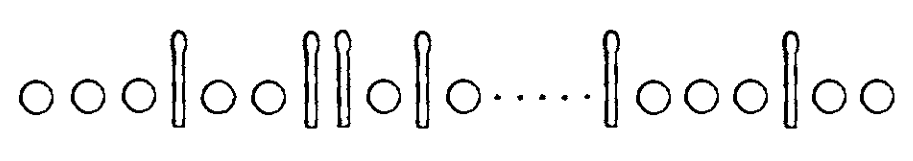
\includegraphics[scale=0.8]{fig15.1.png}
	\figcaption{\sout{黑板上的}排列组合问题:将$U/(\hbar \omega_0)$个相同的小球放入$3 \tilde{N}$个不同的盒子,计算有多少放法。}
	\label{fig15.1}
}

这个组合问题可以这样解决。假设有$U/(\hbar \omega_0)$个相同的小球以及$3 \tilde{N} - 1$根火柴棒,我们试着将它们以任意顺序排成一排。图15.1是其中一种排法,它对应的分布是:第1个模式有3个能量量子(小球)、第2模式有2个、第3模式没有,等等等等,最后一个(第$3 \tilde{N}$个)模式的有2个量子。因此将$U / (\hbar \omega_0)$个量子分布到$3 \tilde{N}$个模式的分布方式数目,等于($3 \tilde{N} - 1 + U/\hbar \omega_0$)个物体(其中有$U/\hbar \omega_0$个相同的小球或能量量子、$3 \tilde{N} - 1$个不同的火柴棒)的置换数,它等于:
\begin{equation}
	\Omega = \frac{(3 \tilde{N} - 1 + U / \hbar \omega_0)!}{(3 \tilde{N} - 1)! (U / \hbar \omega_0)!} \approx \frac{(3 \tilde{N} + U / \hbar \omega_0)!}{(3 \tilde{N})! (U / \hbar \omega_0)!}.
\label{equ15.2}
\end{equation}
这样就算得差不多了,对$\Omega$取自然对数再乘$k_B$就得到了熵。为了简化结果,我们利用大数对数的近似式——Stirling公式:
\begin{equation}
	\ln (M!) \approx M \ln M - M + \cdots \quad (\text{if}\ M \gg 1).
\label{equ15.3}
\end{equation}
算得系统的摩尔熵为:
\begin{align}
	s &= 3R \ln \left( 1 + \frac{u}{u_0} \right) + 3R \frac{u}{u_0} \ln \left( 1 + \frac{u_0}{u} \right). \label{equ15.4} \\
\intertext{其中}
	u_0 &\equiv 3N_A \hbar \omega_0. \label{equ15.5}
\end{align}
这就是系统的基本方程。

验证这个基本方程的靠谱性——也就是验证该方程蕴含着系统合理的热力学性质——的工作留作习题。从中可以导出,系统的摩尔热容在绝对零度为零,并且随着温度的升高而快速增加,直到在高温区域达到常量$3R$,这与实验定性地符合。而热容的增长率与实验在定量上符合的不好,因为这个模型关于振动模式的假设太简化了。在采用更实际的方法处理振动模式之后,这个模型就进化为“Debye模型”(见\ref{sec16.7}节)。

Einstein模型中热容关于温度的关系如图15.2所示。可见摩尔热容$c_v$在$T = 0$处等于0,并且在高温处渐进于常量$3R$. $c_v$在温度为$k_B T \approx \dfrac{1}{3} \hbar \omega_0$区域开始上升($c_v / 3R = \dfrac{1}{2}$以及曲线变化率最大的位置都在$k_B T / \hbar \omega_0 \approx \dfrac{1}{3}$附近)。在低温区,$c_v$随温度以指数方式降低,但实验表明$c_v$大致以$T^3$降低。

{
	\centering
	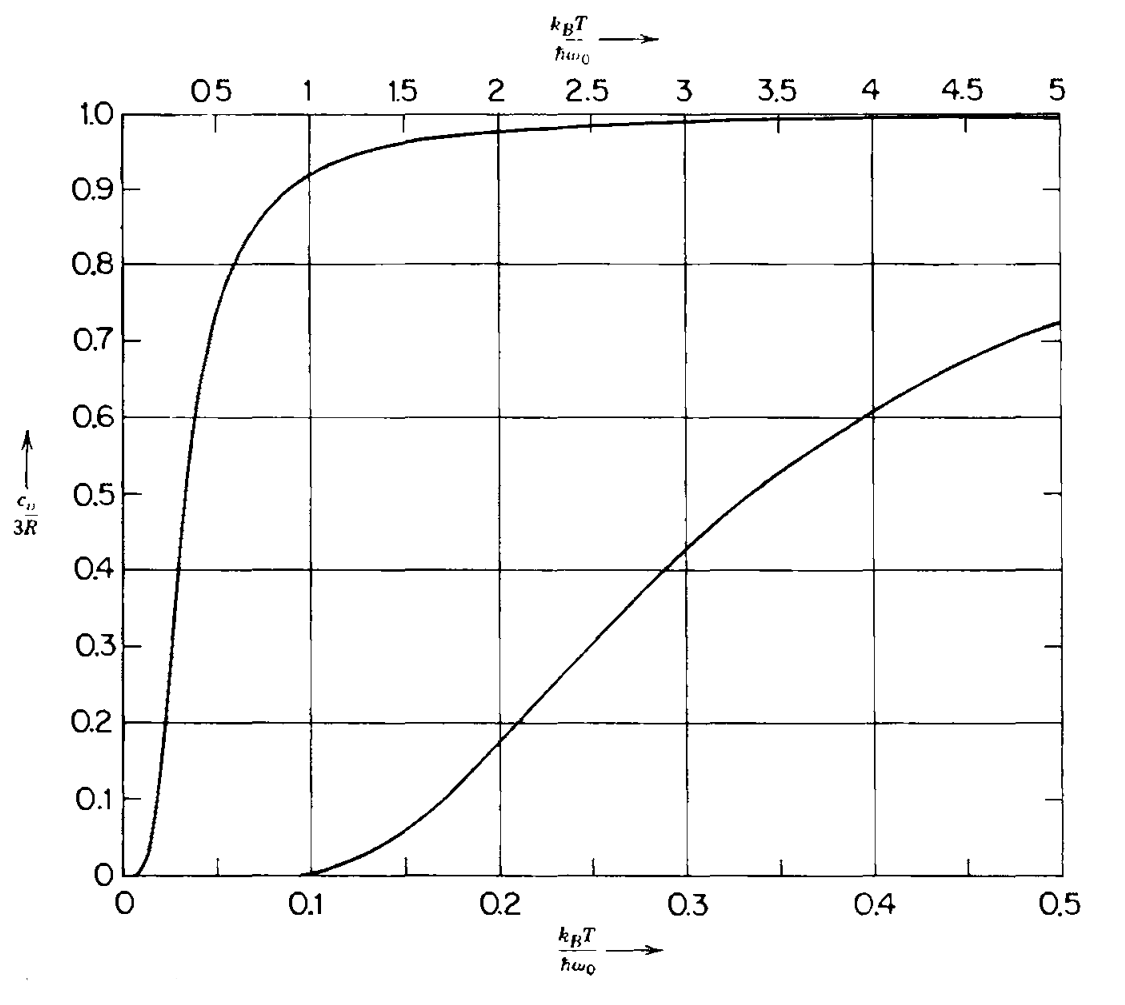
\includegraphics[width=\textwidth]{fig15.2.png}
	\figcaption{Einstein模型的(单个谐振子)系统热容。上面的曲线对应$k_B T / \hbar \omega_0$的上方标度,上面的曲线对应$k_B T / \hbar \omega_0$的下方(拉开了的)标度。纵坐标既可以看成单个谐振子的热容(单位为$k_B$),也能看作系统的摩尔热容(单位为$3R$)。}
	\label{fig15.2}
}

这个模型的力学性质预言——压强-体积关系、压缩率等等——是完全不靠谱的。根据\eqref{equ15.5}式,系统的熵与体积无关,于是压强$P = T \partial S / \partial V$恒为零!这样一个不现实的结论是模型简单地忽略依赖体积的物理效应的结果。

Einstein模型的某些推论含意深远。考虑热状态方程:
\begin{equation}
	\frac{1}{T} = \frac{\partial S}{\partial U} = \frac{k_B}{\hbar \omega_0} \ln \left(1 + \frac{3N}{U} N_A \hbar \omega_0 \right).
\label{equ15.6}
\end{equation}
考虑到系统有$3 N N_A$个谐振子,于是:
\begin{equation}
	\text{谐振子的平均能量} = \frac{U}{3N N_A} = \frac{\hbar \omega_0}{\exp \left( \dfrac{\hbar \omega_0}{k_B T} \right) - 1}.
\label{equ15.7}
\end{equation}
$\hbar \omega_0 / k_B$称为晶体的“Einstein温度”,它通常与固体的熔化温度的数量级相同。因此在低于融化温度时,谐振子的平均能量小于等于$\hbar \omega_0$的量级。换言之,固体在Einstein谐振子的量子数显著高于基态之前熔化。

\subsection*{习题}
\begin{itemize}
	\item[15.2-1.] Calculate the molar heat capacity of the Einstein model by equation \eqref{equ15.7}. Show that the molar heat capacity approaches $3R$ at high temperatures. Show that the temperature dependence of the molar heat capacity is exponential near zero temperature, and calculate the leading exponential term.
	\item[15.2-2.] Obtain an equation for the mean quantum number $\bar{n}$ of an Einsten oscillator as a function of the temperature. Calculate $\bar{n}$ for $k_B T / \hbar \omega_0 = 0, 1, 2, 3, 4, 10, 50, 100$ (ignore the physical reality of melting of the crystal!).
	\item[15.2-3.] Assume that the Einstein frequency $\omega_0$ for a particular crystal depends upon the molar volume:
	\[
		\omega_0 = \omega_0^0 - A \ln \left( \frac{v}{v_0} \right).
	\]
	\begin{itemize}
		\item[(a)] Calculate the isothermal compressibility of this crystal.
		\item[(b)] Calculate the heat transfer if a crystal (of one mole) is compressed at constant temperature from $v_i$ to $v_f$.
	\end{itemize}
\end{itemize}

\section{双态系统}
\label{sec15.3}
